\documentclass[a4paper,12pt]{article}
\usepackage[T1]{fontenc}
\usepackage[latin9]{inputenc}
\usepackage{listings}
\usepackage{amsmath}
\usepackage{mathtools}
\usepackage{mathpazo}
\usepackage{wasysym}
\usepackage{graphicx}
\usepackage{tikz,pgfplots}
\usepackage[colorinlistoftodos]{todonotes}
\usepackage{natbib} 
\usepackage{geometry}
\usetikzlibrary{fit,shapes.misc,snakes}
\geometry{verbose,tmargin=2.5cm,bmargin=2.5cm,lmargin=2.5cm,rmargin=2.5cm}

\newcommand{\ord}{\operatorname{ord}}

\begin{document}

\title{Algorithm Engineering\\Project 2}

\author{Lasse Espeholt - 20093223\\
Kasper Nielsen - 20091182}

\maketitle

\includegraphics[width=\textwidth]{"images/forside"}

\vfill{}
\begin{description}
\item [{Implementation~code~and~test~results:}] \texttt{http://github.com/kasper0406/AlgEng/project2}
\end{description}
\pagebreak{}\tableofcontents{}\pagebreak{}

\section{Introduction}
The purpose of the following rapport is to demonstrate that the complexity of algorithms depends heavily on the hardware the algorithms are running on. Cache faults, branch predictions etc. influences the performance to a great degree.

The problem under test is a set $S$ containing $N$ integers which supports the following query:

\begin{eqnarray*}
\mathrm{Pred}(x) = \max \{ y \in S\ |\ y \leq x \}
\end{eqnarray*}

\section{Algorithms and data structures}
In this section we will describe the different algorithms and memory
layouts we have used.

\subsection{Simple multiplication}

\subsubsection{Row-based layout}
We started out implementing the simple conventional $O(n^3)$ matrix
multiplication algorithm where we stored the matrices using a row
based layout.

In order to estimate the number of cache faults, we will for each row
in the output matrix try to bound the number of cache faults
encountered in order to compute it. We assume that the cache is reset
after the computation of a row\todo{Argue why this makes sense}.

\todo{Insert image illustrating this!}
When computing a row in $C = AB$, we keep a row in $A$ fixed, and vary
the columns in $B$. Hence the row i $A$ will always be in cache,
initially causing $\frac{n}{B}$ cache faults. We compute all columns
in the result row sequentially. Because our cache is big enough to
hold $n+1$ cache lines\todo{Argue!?}, we can hold all cache lines


\todo{Expectations of cache faults here....}

We do not expect any significant amount of branch mispredictions.

\subsubsection{Combined row-based and column-based layout}

In order to improve the number of cache faults, we have tried to use a
column base layout in the right operand in the multiplication. We
expect this to give us a bit better cache performance. This approach
has the drawback of limiting a matrix only to be used on one side of a
multiplication. However, this problem can be mitigated by conversions which is an $O(n^2)$ operation.

We analyze the number as cache faults as before, but 

\subsection{Recursive multiplication}

For exploiting more kinds of layouts we implemented the recursive algorithm.

\subsubsection{Z-curve layout}

The first idea was to use a Z-curved layout. One major advantage of this layout is that improves locality on all levels of the recursive multiplication. The drawback is that the index calculations are time consuming. On x86 we get approximately 50 bitwise operations each time we want to convert a coordinate to the position in the array. However, this can be improved by incrementally constructing the Z-curve numbers or by precomputing offsets at base cases. The upcoming Intel Haswell architecture has support for bit permutations which will improve the situation.

We ended up with precomputing the Z-curve offsets at the base case. That means the only penalty when we want to store or lookup a value is a level of indirection. In the recursive algorithm we used 8*8 as a base case for switching to the naive algorithm.

\subsubsection{Tiled layout}

A tiled layout is a compromise between locality and performance of index calculations. When the recursive algorithm reaches blocks of the same size as the tiles, it switches to the naive algorithm. And the naive algorithm functions without any modifications. To improve cache locality a bit we used a row-based layout in the tiles for the left operand and a column-based layout in the tiles for the right operand.

\subsection{Strassen}

Strassen exploits some tricks with matrix multiplication such that it only uses 7 multiplications instead of 8 multiplications. It is a recursive algorithm by nature. The first step of the algorithm is the split the operands into 2*2 blocked matrix.

Instead of actually splitting the matrix into smaller matrices we have used a Z-curve layout. That means that the smaller matrices are able to just point to the data in the parent matrix while still preserving a proper layout themselves.

Strassen needs to have a large base case such that we do not spend too much time on the recursion and to improve cache locality at the base levels. To avoid the overhead of handling matrix multiplication with a level of indirection or by calculating Z-curve indices, we used a row-based and column-based layout at the base case for the left and right operand respectively.

The additions and subtractions in the algorithm only works on left operand block matrices or right operand block matrices. Therefore, we can use a single loop and no index calculations to add and subtract matrices. I.e. Z-curve indices are the same and we only add/subtract row-based base cases with row-based base cases etc.

\todo{Manglende praecision}

\subsection{Special instructions}

...

\subsection{Parallelization}

\subsubsection{Combined row-based and column-based layout}

The naive algorithm which is used for this combined is easily parallelizable because we can assign intervals of rows for each thread. The result matrix is stored in a row-based layout so writing is separated so cache thrashing should not be a problem.

...

\todo{todo, mere l2 cache}

\todo{formelen for parallelization}

\subsubsection{Strassen}

Strassen was parallelized by starting new threads at each of the 7 multiplications. This was done at 1 or 2 levels depending on the level of parallization we wanted. The last additions/subtractions and combine operations were not parallelized. However, the multiplications uses most of the time.

\clearpage{}
\section{Benchmarks}
\subsection{Test setup}

Our program was written in C/C++ and compiled with Clang. All memory allocations were cache line boundary aligned. For parallelization we used C++11 cross-platform library \texttt{<thread>}.

All benchmarks were performed on a Linux desktop which has 4 GB ram and a Core i3 550 CPU with the following specification:

\begin{itemize}
\item 2 * 3.2 GHz (no Turbo boost)
\item 2 * 32 KB L1 instruction cache
\item 2 * 32 KB L1 data cache
\item 2 * 256 KB L2 cache
\item Shared 4 MB L3 cache
\item 64 byte cache lines
\item Inclusive caches
\item The associativity for the cache levels are 8, 8 and 16 respectively
% http://www.ni.com/white-paper/11266/en#toc5
\end{itemize}

L2 cache faults and L3 cache faults were measured using Intel Performance Monitor Counter while branch mispredictions were measured using PAPI.

All tests were performed 5 times and the median was selected. The data in the matrices were randomly generated double precision floating points with
an uniform distribution. The range of the data was -1 to
1.

\subsection{Simple multiplication}

\subsubsection{Row-based layout}
Figure~\ref{fig:rnrnrn0} shows the measured running time and cache
faults encountered when running the naive matrix multiplier on
matrices with row layout.
\begin{figure}[h!]
  \centering
  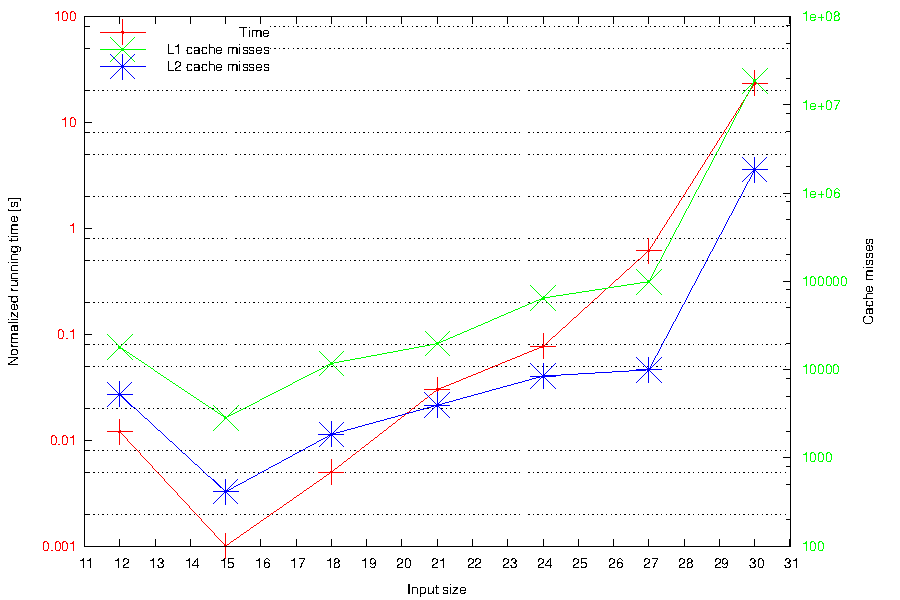
\includegraphics[width=\textwidth]{rnrnrn0.pdf}
  \caption{Running time and cache faults of naive matrix
    multiplication with all matrices using row layout.}
  \label{fig:rnrnrn0}
\end{figure}

As it can be seen in the plot, we start out by approximately the
expected number of L2 and L3 cache faults. However, the number of L2
cache faults quickly explodes, and the number of L3 cache faults also
far exceeds out expectations. It seems like the L2 cache begins to
perform very badly between instances of size $2^7 = 128$ and $2^8 =
256$, and that the L3 cache loose its performance when going from
$2^{9} = 512$ to $2^{10} = 1024$.

We highly suspect that the cache layout due to the 8-way associativity
is to blame. When looking up in the L2 cache, the 36 bit physical
address of the i7 processor is split into three parts $addr =
(tag,index,offset)$. Since the cache line size is $64b$, $6$ bits
should be used to reference a byte in a cache line. Because the L2
cache is $256kb$, we find that the index size to be
\[
  \frac{256 \cdot 1024}{\underbrace{64}_{\text{Cache line size}} \cdot \underbrace{8}_{\text{Cache associativity}}}
    = 512 = 2^9.
\]
Hence, we should use $9$ bits to specify the index. The remaining
$36-6-9=21$ bits is used as tag. Notice that the tag is the most
significant part of the address.

Because our matrices are square matrices of size a power of two, it
will always be the case that a new row in a matrix starts with a new
cache line. But this means that a cache line, and the corresponding
cache lines on the next row, always will be $\frac{n}{B}$ cache lines
apart. Therefore, when we read a matrix with row layout in a column
like fashion, we can only use $\frac{2^9}{\frac{n}{B}} =
\frac{2^9B}{n}$ cache lines. Since the L2 cache i 8-way associative,
we have to write to each entry before we begin to trash the cache
lines. Therefore we find that
\[
\frac{2^9 B}{n} \cdot \overbrace{8}^{\mathclap{\text{8-way associativity}}} \leq n
\iff
181 \approx \sqrt{2^9 \cdot 8^2} \leq n.
\]
When we exceed this number we should switch to our bad-case analysis
from the algorithms section. This switch occurs a lot earlier than
expected (the expected was $n$ around $2000$), because of the way the
cache is structured. Observe that this analysis predicts that we will
begin to trash the L2 cache between $n = 128$ and $n = 256$. This is
exactly what is measured in our experiments.

A similar analysis can be made for the L3 cache. It is a $16$-way
cache having $8$ megabytes of storage. This gives an index size of
$2^{13}$. Therefore we find that
\[
\frac{2^{13} \cdot B}{n} \cdot 16 \leq n \iff 1024 = \sqrt{2^{13} \cdot 8 \cdot 16} \leq n
\]
This is also where our experiments shows that the L3 cache begins to
trash it's values.

Figure~\ref{fig:rowrowfixed} shows a plot with the updated
expectations. It can be seen that these fits quiet good with our
measurements.
\begin{figure}[h!]
  \centering
  \missingfigure{Cache faults on naive row-row layout with updated expectations.}
  \caption{Cache faults on naive row-row layout with updated
    expectations.}
  \label{fig:rowrowfixed}
\end{figure}

\subsubsection{Combined row-based and column-based layout}

\ref{fig:rncnrn0}

\begin{figure}[h!]
  \centering
  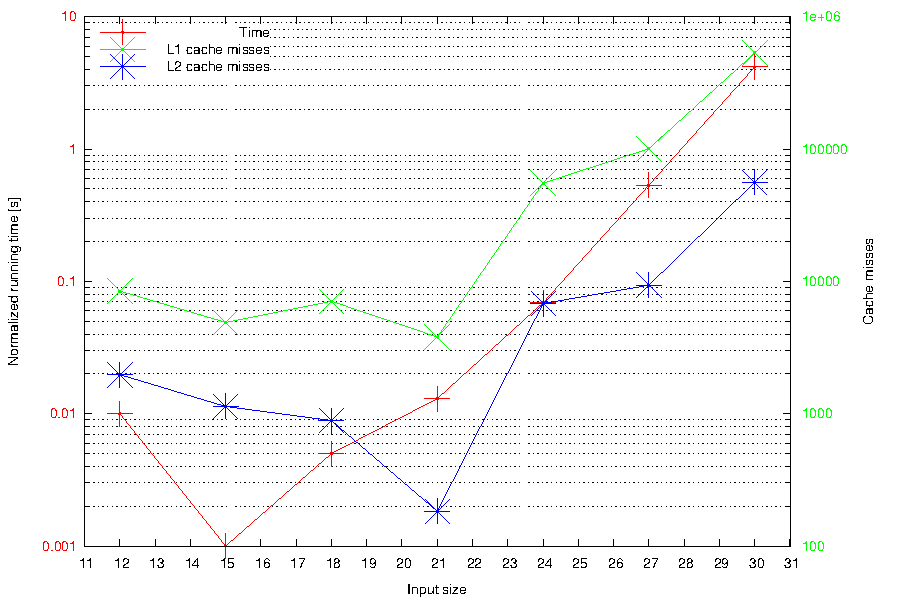
\includegraphics[width=\textwidth]{rncnrn0.pdf}
  \label{fig:rncnrn0}
\end{figure}

\subsection{Recursive multiplication}

\subsubsection{Z-curve layout}

\ref{fig:zrzrzr0}

\begin{figure}[h!]
  \centering
  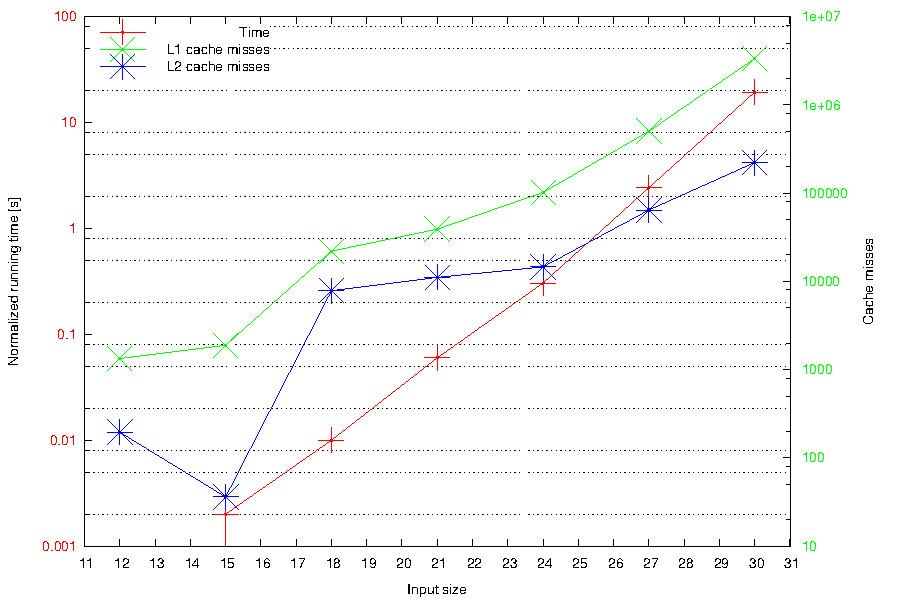
\includegraphics[width=\textwidth]{zrzrzr0.pdf}
  \label{fig:zrzrzr0}
\end{figure}


\section{Conclusion}
\begin{figure}[h!]
  \centering
  \includegraphics[width=\textwidth]{"../project2/gnuplots/best_single"}
  \label{fig:best_single}
  \caption{Summarised single-core performance.}
\end{figure}

\begin{figure}[h!]
  \centering
  \includegraphics[width=\textwidth]{"../project2/gnuplots/best_parallel"}
  \label{fig:best_parallel}
  \caption{Summarised multi-core performance.}
\end{figure}

\todo{Opsummering af algoritmer og hvordan de har klaret sig}

\todo{Layout rigtig vigtig}

\todo{Strassen, numerisk stabilitet samt ikke ligesaa god til parallisering => iterativ god}

\todo{Alt i alt, ved at benytte layout, algoritmer, simd, paral. saa har vi faaet noget der er langt bedre}

\clearpage{}\bibliographystyle{plain}
\addcontentsline{toc}{section}{\refname}\bibliography{ref}

\end{document}
